% ********** Rozdział 3 **********
\chapter{Harmonogram realizacji projektu}

Harmonogram realizacji projektu "System zarządzania kontem klienta w firmie telekomunikacyjnej" został stworzony w celu zaplanowania i kontrolowania procesu implementacji systemu oraz jego poszczególnych funkcjonalności. Harmonogram obejmuje szereg etapów, w których uwzględniono zadania związane z analizą wymagań, projektowaniem, implementacją, testowaniem i wdrożeniem systemu.

\section{Diagram Gantta}
\begin{figure}[h]
    \centering
    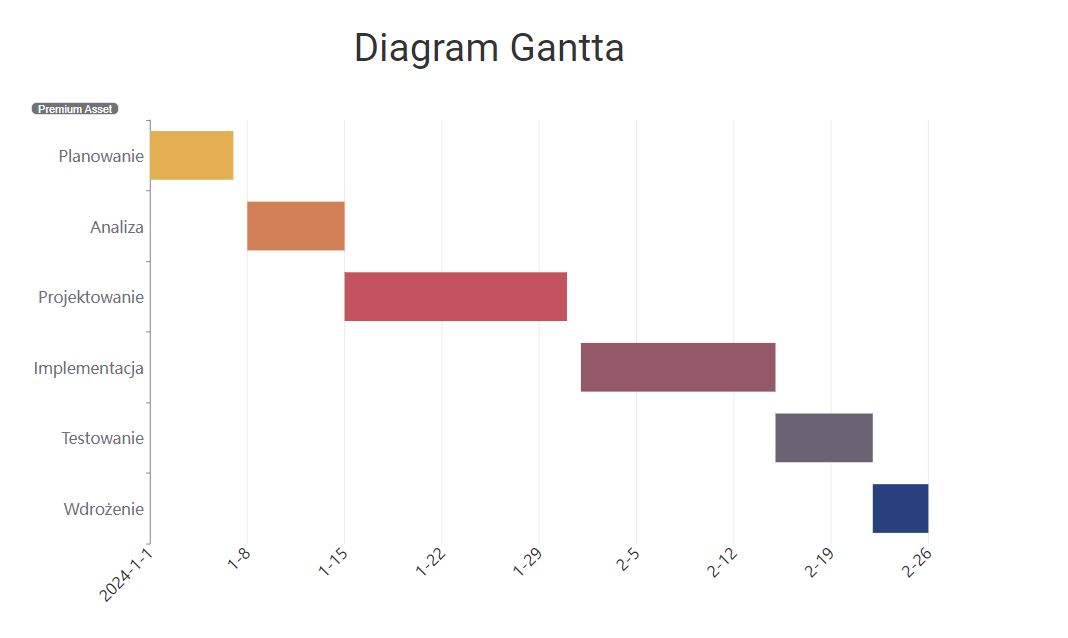
\includegraphics[width=\textwidth]{Gantt.png}
      \caption{Diagram Gantta - Opis realizacji projektu}
    \label{fig:example}
\end{figure}

\newpage

\subsection{Projektowanie (1/01/2024 - 7/01/2024)}
\begin{itemize}
    \item Zdefiniowanie funkcjonalnych i niefunkcjonalnych wymagań systemu.

\end{itemize}

\subsection{Analiza (8/01/2024 - 15/01/2024)}
\begin{itemize}
    \item Określenie oczekiwanych funkcji i interfejsu użytkownika
\end{itemize}

\subsection{Projektowanie (15/01/2024 - 31/01/2024)}
\begin{itemize}
    \item Opracowanie architektury systemu i struktury bazy danych.
    \item Utworzenie diagramów klas, schematów bazodanowych oraz interfejsów użytkownika.
    \item Sporządzenie dokumentacji projektowej i specyfikacji technicznej.
\end{itemize}

\subsection{implementacja (1/02/2024 - 15/02/2024)}
\begin{itemize}
    \item Pisanie kodu.
    \item Wprowadzanie poprawek do kodu i implementowanie kolejnych funkcjonalności.
\end{itemize}

\subsection{Testowanie (15/02/2024 - 22/02/2024)}
\begin{itemize}
    \item Przeprowadzenie testów funkcjonalnych i niefunkcjonalnych.
    \item Debugowanie i poprawa ewentualnych błędów.
\end{itemize}

\subsection{Wdrożenie (22/02/2024 - 26/02/2024)}
\begin{itemize}
    \item Prowadzenie testów integracyjnych i ostateczne dostosowanie systemu.
\end{itemize}

Harmonogram realizacji projektu jest elastyczny i może ulec zmianie w razie konieczności dostosowania do zmieniających się warunków lub potrzeb projektowych.


% ********** Koniec rozdziału **********
